
\section{Trigonometry}

\subsection{Problems}

\begin{center}
    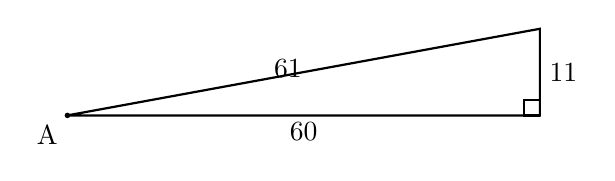
\begin{tikzpicture}
        % Define the coordinates of the triangle
        \coordinate (A) at (0,0);
        \coordinate (B) at (6,0);
        \coordinate (C) at (6,1.1);
        
        % Draw the triangle
        \draw[thick] (A) -- (B) -- (C) -- cycle;
        
        % Mark the right angle
        \draw[thick] (B) -- ++(-0.2,0) -- ++(0,0.2) -- ++(0.2,0);
        
        % Label the sides
        \node at (3,-0.2) {60};
        \node at (6.3,0.55) {11};
        \node at (2.8,0.6) {61};
        
        % Label the points
        \node[below left] at (A) {A};
        
        % Mark the points
        \fill (A) circle (1pt);
    \end{tikzpicture}
\end{center}

\bigskip

Choose the correct answer:

\[
\begin{aligned}
    \text{A) } & \quad \sin A = \frac{61}{11} \\
    \text{B) } & \quad \sin A = \frac{60}{61} \\
    \text{C) } & \quad \sin A = \frac{11}{61} \\
    \text{D) } & \quad \sin A = \frac{11}{60}
\end{aligned}
\]

\footnote{Source: Math10, \emph{Trigonometry Problems}, \url{https://www.math10.com/problems/trigonometry-problems/easy/}}

